% !TEX root = mainthesis.tex

%Chapter 4


\renewcommand{\thechapter}{4}


\chapter{Making BECs in the Rubidium Lithium apparatus}

All the experiments presented in this thesis were performed at the Rubidium-Lithium (RbLi) apparatus at the University of Maryland. The experiment was designed to produce mixtures of quantum degenerate gases of bosons and fermions. The original plan was abandoned because the cross-species scattering length was found to be repulsive and small ($a_s\approx20\,a_B)$~\cite{silber_quantum-degenerate_2005} and the nearest heteronuclear $s$-wave Feshbach resonance was measured to occur at the unexpectedly large magnetic field of $\unit[1066]{G}$~\cite{deh_feshbach_2008} and therefore all our experiments were performed using only $\Rb87$.

As of the time this thesis is being written, the apparatus is scheduled to be shut down and the construction of a new dual-species apparatus for $\Rb87$ and K$^{39}$ is underway. I will not describe in detail the technical details of the RbLi apparatus which have been extensively discussed in the theses of former lab members~\cite{CampbellThesis,PriceThesis}. I will describe the experimental sequence that we follow to achieve BEC. Where it is relevant I will comment on some troubleshooting techniques that were helpful to us as well as on particular pieces of hardware that work either exceptionally well or exceptionally poorly. The outstanding elements of the lab are summarized in Table \note{TODO: make table of best and worst of RbLi}. Additionally in Appendix~\ref{app:Basement_lab} I will describe technical aspects of the construction of the new apparatus where I was involved. 


\section{Creating an atomic beam}

The RbLi vacuum system has a dual species oven designed for both Rb and Li. Both Rb and Li atoms are heated up. The Rb oven was kept at $\unit[120]{C}$ while the Li oven at $\unit[160]{C}$, below the temperature required to make an atomic beam. The heated atoms travel to the main oven chamber that is pictured in Figure~\ref{fig:RbLi}b containing a cold-cup and an oven shutter. The cold-cup is a cylindrical shaped copper piece that is attached to the cold end of a thermo-electric cooler (TEC) via a copper rod. We keep the cold-cup temperature at $-\unit[30]{C}$ in order to capture excess Rb atoms in the chamber and prevent damaging the ion pumps. On January 2018 we noticed that an excessive buildup of Rb atoms in the cold cup was blocking the atomic beam. To remedy this issue we closed the gate valve between the oven and the Zeeman slower to make sure the UHV portion stayed clean. We then reversed the polarity of the TEC that we heated the cold cup just enough to see the Rb atoms melt and clear the path of the atomic beam. Finally we cooled the TEC back to $\unit[-30]{C}$ and waited a full day before opening back the gate valve. We have been able to successfully operate the experiment without any vacuum related problems after this procedure was performed. 

\begin{figure*}[htb]
\begin{center}
\includegraphics[]{Figures/Chapter4/RbLi.pdf}
\caption[The RbLi vacuum system]{$\Rb87$ level structure (not to scale). {\bf a.} Ground and first excited state electronic configuration of $\Rb87$ given by the $\{n,\mathbf{L}\}$ quantum numbers. {\bf b.} The interaction between the orbital angular momentum and the spin of the electron leads to the fine splitting of orbitals with $L>0$. The splitting of the $5^2P$ line gives rise to the D1 and D2 lines. {\bf c.} The interaction between the total angular momentum and the nuclear spin causes the fine structure levels to split further into states characterized by the quantum number $F$.}
\label{fig:RbLi}
\end{center}
\end{figure*}

The oven shutter allows us to block or enable the atomic beam. We use a homemade device, made from a re-purposed hard drive disk shutter with a metallic flag attached to its end. The shutter is electrically connected to en electric feedthrough with vacuum-compatible Kapton sealed wires. We never experienced any trouble with our shutter, unlike one other apparatus~\cite{BrownThesis} within the JQI which used a \noted{Uniblitz} commercial shutter that failed and had to be replaced. 


\section{Magneto-optical trap and subdopler cooling}

From the oven chamber the atomic beam travels down a Zeeman slower~\cite{phillips_laser_1982 } (see Figure~\ref{fig:RbLi}a) where atoms are laser cooled. The Zeeman slower additionally acts as a differential pumping stage between the oven side and the ultra-high vacuum (UHV) side. The UHV side has a glass cell (Figure~\ref{fig:RbLi}a,c) where we trap and laser cool atoms in a magneto-optical trap (MOT).

\subsection{Magnetic field control}
The Zeeman slower and quadrupole coils (used for the MOT and magnetic trapping later in the sequence) are operated at relatively high currents. The coils are connected in series with MOSFET banks, each one sharing the same gate voltage that is controlled by a PI servo. The Zeeman slower always operates at a fixed current but the current in the quadrupole coils is dynamically changed throughout the experimental sequence and a fast response is desirable. In 2013 we replaced the quadrupole MOSFET bank with a new unit that contains 20 \noted{IXFN 520N075T2} transistors rated for $\unit[75]{V}$ and $\unit[480]{A}$ that are shown in Figure xxx. The use of more transistors reduces the power dissipation of each individual transistor which allows us to operate the power supply at a higher voltage of $\unit[15]{V}$ that helps counteract the inductive kickback of the coils. With the new transistor bank the turn on time of the coils was reduced from $\unit[100]{ms}$ to $\unit[50]{ms}$ leading to improved magnetic trapping and better Stern-Gerlach pulses for imaging.

We additionally use bias coils that generated uniform magnetic fields along $\ex$, $\ey$, and $\ez$. The coils are driven using \noted{Kepco BOP} $\unit[\pm20]{A}$ power supplies. The Kepcos have been a standard equipment in our group but they are not cheap, their output has a lot of $\unit[60]{Hz}$ noise, and tend to fail in various annoying ways (burnt transistors, broken switches,...). Our group is currently working on designing a homemade bipolar power supply based on a combination of N-type and P-type MOSFETS and opamps \note{TODO: ask Mingshu}.  

\subsubsection{Water cooling of coils}
The quadrupole and Zeeman slower coils as well as the transistor banks require water cooling due to Joule heating. Our lab space is shared with a Rubidium-Ytterbium ultracold mixtures apparatus~\cite{HeroldThesis} and amongst the things we shared is the water cooling system. The schematic in Figure~\ref{fig:water_cooling} illustrates the layout of the water cooling system and one of its failure modes. A $\unit[20]{kW}$ \noted{Coherent LaserPure20} heat exchanger provides chilled water to both experiments. The output of the heat exchanger is split into two lines which provide cooling for both apparatus. A \noted{Berkeley MGPS7D} booster pump provides the high pressure necessary for our coils which have a relatively large impedance. The water returning to the heat exchanger is filtered with a low-impedance cellulose cartridge (\noted{McMaster 7191K11}). One big failure mode of this design occurs when one of the booster pumps is turned on before the heat exchanger, causing water to flow from one experiment to the other and bringing a collection of nasty things that escapes the filters into the coils. Over the years our system has suffered of clogged filters, clogged coils and broken booster pumps. For best operation it is highly recommended that the filter is changed every year and that the a $10\%$ solution of an anti-corrosive \noted{Optishield Plus} in water is used as a coolant\footnote{Even in this case we managed to find lots of gunk and unidentified objects (sand? glass? mud? oxide?) in the water}. 

\begin{figure*}[htb]
\begin{center}
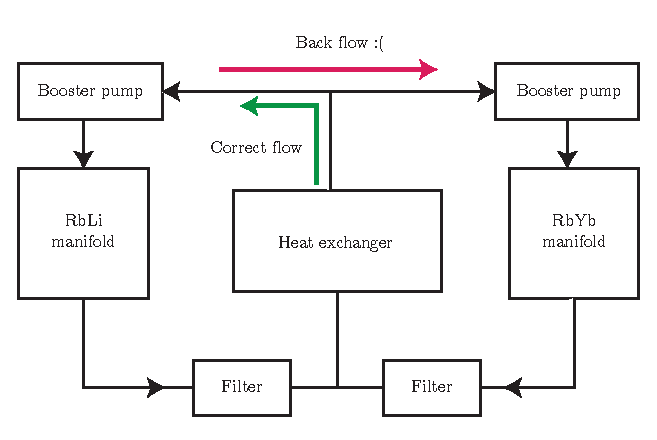
\includegraphics[]{Figures/Chapter4/water_cooling.pdf}
\caption[Water cooling manifold schematic]{\note{TODO: write caption for plumbing figure.}}
\label{fig:water_cooling}
\end{center}
\end{figure*}

\subsection{Computer control and data acquisition}
\begin{figure*}[htb]
\begin{center}
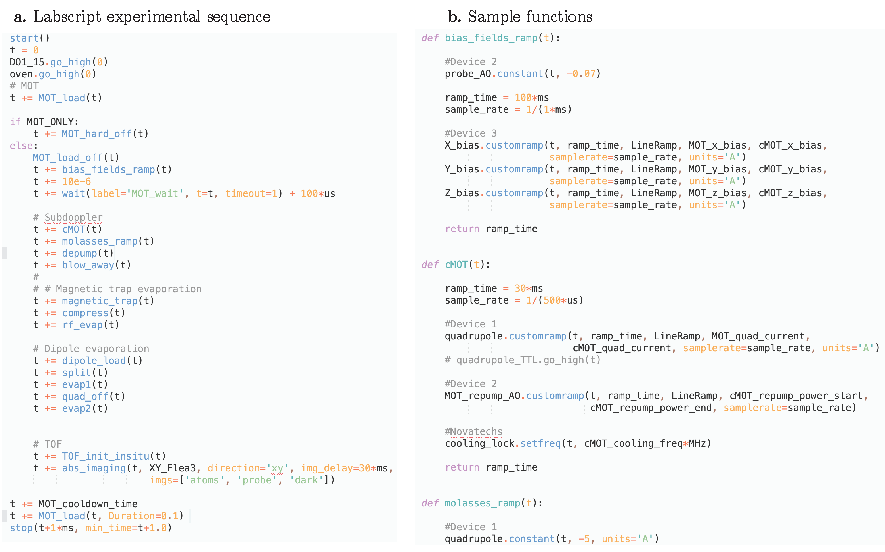
\includegraphics[]{Figures/Chapter4/labscript.pdf}
\caption[Water cooling manifold schematic]{\note{TODO: write caption for plumbing figure.}}
\label{fig:labscript}
\end{center}
\end{figure*}

\subsection{Laser systems}

We used a total of three lasers to perform laser cooling of atoms: a cooling laser that addresses the $F=2\rightarrow F'=3$ transition, a repump laser that takes atoms that have decayed into the $F=1$ state back to $F=2$ and a master laser that provides a frequency reference for both lasers. 

The frequency of master laser is locked using saturation absorption spectroscopy to the $F=3\rightarrow F'=3$ and $F=3\rightarrow F'=4$ crossover of the D2 line of $^{85}$Rb. Previously we used a \noted{New Focus Vortex II TLB-6900} extended cavity diode laser as our master laser and a home made saturation spectroscopy setup using a Rb glass cell (see~\cite{CampbellThesis,PriceThesis}). The frequency of this laser turned out to be extremely unstable and was replaced by a \noted{Vescent photonics DBR Laser Moduee System} which uses a distributed Bragg reflector laser diode with no external cavity and is therefore very mechanically stable. The frequency of the laser is stabilized and controlled using the \noted{D2-210} spectroscopy module and \noted{D2-125} laser servo. The master laser system is considerably simplified as can be seen in Figure~\ref{fig:master_laser}.

\begin{figure*}[htb]
\begin{center}
\includegraphics[]{Figures/Chapter4/master_laser.pdf}
\caption[Water cooling manifold schematic]{\note{TODO: write caption for plumbing figure.}}
\label{fig:master_laser}
\end{center}
\end{figure*}

The cooling laser system consists of a \noted{Toptica DL Pro}. A small fraction of the light is used in the beatnote lock and and for imaging probe beams, the remaining fraction is amplified using a \noted{Toptica BoosTA} tapered amplifier system. The output of this TA system has been very stable over the years and there has not been a considerable decay in power over more than 6 years. However, this TA system can be a bit temperamental and shuts itself off. We have developed a turn-on procedure that increases the current in $\unit[100]{mA}$ steps every $\unit[10]{s}$. Turning it on at full current in a single step is a known cause of TA suicide, other causes are still unknown despite our best efforts to figure it out.

The repump laser system is the same model \noted{Toptica DL Pro} as the cooling laser. However, it is not nearly as stable. In particular, it takes a lot of time to stabilize after turn-on and it tends to mode hop or to have a multi-mode output. 

-Flipper mirrors suck
-Polarimeter and PD for MOT diagnostics


\cite{anderson_loading_2001}

\subsubsection{Dipole laser}
We use a $\unit[30]{W}$ \noted{IPG Photonics} $\unit[1064]{nm}$ laser to generate dipole traps for the atoms. The laser system is not fiber coupled and is setup in the same optical table as the vacuum system;  we are not able to change the laser without destroying the alignment of the beam with the atoms. In the original design of the laser system high-power photonic crystal fibers were included but they did not have built in mode expanders which resulted in the tip of the fiber inevitably getting burnt after some time of use. This will be remedied in the new apparatus which will have a fiber coupled dipole trap using high-power optical fibers with mode expanders from \noted{Coastal Connections}. \note{TODO: ask Junheng for part number.}

\subsubsection{Raman laser}

\subsubsection{A note on PM optical fibers}

Here talk about fiber paddles and fiber splitter



\subsection{XY imaging system}
-Mako camera is awesome





\subsection{High power RF antenna}
\label{sec:high_power_rf_antenna}
The antenna loop is Digikey part number $732-5646-ND$


\subsection{Computer control and data acquisition}
Labscript is awesome. 


\section{Experimental sequence to make BECs}
\label{sec:making-becs}

\subsection{MOT}



\subsection{Adiabatic rapid passage}
\label{sec:arp}
-Trigger to the 60Hz line is essential. 

\subsection{Magnetic field stabilization with microwaves and partial transfer absorption imaging}
\label{sec:ptai}
We then apply a pair of $250\,\mu\mathrm{s}$ microwave  pulses that each transfer a small fraction of atoms into the $5^2{\rm S}_{1/2}$ $f=2$ manifold that we use to monitor and stabilize the bias field \cite{leblanc_direct_2013}. The microwave pulses are detuned by $\pm 2\, \kHz$ from the $\ket{f=1,m_F=0}\leftrightarrow\ket{f=2,m_F=1}$ transition and spaced in time by $33\, \mathrm{ms}$ (two periods of $60\, \mathrm{Hz}$). We imaged the transferred atoms following each pulse using absorption imaging\footnote{We did not apply repump light during this imaging, so the untransferred atoms in the $f=1$ manifold were largely undisturbed by the imaging process.}, and count the total number of atoms $n_1$ and $n_2$ transferred by each pulse. The imbalance in these atom numbers $(n_1-n_2)/(n_1+n_2)$ leads to a $4\kHz$ wide error signal that we use both to monitor the magnetic field before each spectroscopy measurement and cancel longterm drifts in the field. 

\section{Recap}

Our current postdoc once said `I love every single thing about RbLi.' 

Make a table with `do', `dont' and `quastionable'

do:
overkill transistor banks
home made in vacuum shutters
fiber paddles
polarizers to clean mot beams
mica capacitors for high power RF impedance matching
labscript
Mako camera
mode expanders on high-power optical fibers
Vescent laser
Lab couch
picomotors

dont:
free space dipole laser
shared water cooling
flipper mirrors

questionable:
kepco
BoosTA
too many NI usb devices on the same computer